\documentclass[12pt, twoside]{report}
\usepackage[a4paper, top=2.0cm, bottom=2.0cm, left=2.5cm, right=2.5cm]{geometry}

\usepackage[MeX]{polski} 
\usepackage[T1]{fontenc}
\usepackage[utf8]{inputenc}
\usepackage{times}
\usepackage{color}
\usepackage{comment}
\usepackage{indentfirst}
\usepackage{graphicx}
\usepackage{mathptmx}
\usepackage{amsmath}
\usepackage{tikz}
\usepackage{hyperref}
\usepackage[final]{pdfpages}
\usepackage{afterpage}
\usepackage{titlesec}
\usepackage{microtype}
\usepackage{enumitem}
\usepackage{caption}
\usepackage{subcaption}
\usepackage{listings}
\usepackage{chngcntr}

\graphicspath{{images/}}
\definecolor{dkgreen}{rgb}{0,0.6,0}
\definecolor{gray}{rgb}{0.5,0.5,0.5}
\definecolor{mauve}{rgb}{0.58,0,0.82}
\definecolor{gray}{rgb}{0.4,0.4,0.4}
\definecolor{darkblue}{rgb}{0.0,0.0,0.6}
\definecolor{lightblue}{rgb}{0.0,0.0,0.9}
\definecolor{cyan}{rgb}{0.0,0.6,0.6}
\definecolor{darkred}{rgb}{0.6,0.0,0.0}

\counterwithin{figure}{section}
\setlength{\parindent}{4em}
\titlespacing{\chapter}{0pt}{-35px}{5px}
\titlespacing*{\subsection}{0pt}{0px}{0px}
\titlespacing*{\subsubsection}{0pt}{0px}{0px}
\titlespacing*{\section}{0pt}{0px}{0px}
       
\titleformat{\chapter}[block]
       {\normalfont\huge\bfseries}{ \thechapter}{15pt}{\Huge}
       
\lstset{
  basicstyle=\ttfamily\footnotesize,
  columns=fullflexible,
  showstringspaces=false,
  numbers=left,                   % where to put the line-numbers
  numberstyle=\tiny\color{gray},  % the style that is used for the line-numbers
  stepnumber=1,
  numbersep=5pt,                  % how far the line-numbers are from the code
  backgroundcolor=\color{white},      % choose the background color. You must add \usepackage{color}
  showspaces=false,               % show spaces adding particular underscores
  showstringspaces=false,         % underline spaces within strings
  showtabs=false,                 % show tabs within strings adding particular underscores
  frame=single,                   % adds a frame around the code
  rulecolor=\color{black},        % if not set, the frame-color may be changed on line-breaks within not-black text (e.g. commens (green here))
  tabsize=2,                      % sets default tabsize to 2 spaces
  captionpos=b,                   % sets the caption-position to bottom
  breaklines=true,                % sets automatic line breaking
  breakatwhitespace=false,        % sets if automatic breaks should only happen at whitespace
  title=\lstname,                   % show the filename of files included with \lstinputlisting;
                                  % also try caption instead of title  
  commentstyle=\color{gray}\upshape
}

\lstdefinelanguage{XML}
{
  morestring=[s][\color{mauve}]{"}{"},
  morestring=[s][\color{black}]{>}{<},
  morecomment=[s]{<?}{?>},
  morecomment=[s][\color{dkgreen}]{<!--}{-->},
  stringstyle=\color{black},
  identifierstyle=\color{lightblue},
  keywordstyle=\color{red},
  morekeywords={xmlns,xsi,noNamespaceSchemaLocation,type,id,x,y,source,target,version,tool,transRef,roleRef,objective,eventually}% list your attributes here
}
\linespread{1.5}

\newcommand\tab[1][0.5cm]{\hspace*{#1}}



\hypersetup{
    colorlinks,
    citecolor=black,
    filecolor=black,
    linkcolor=black,
    urlcolor=black
}

\newcommand\blankpage{%
	\null
    \thispagestyle{empty}%
    \newpage}

\pdfinfo{
   /Author (Krzysztof Dragan)
   /Title  (Aplikacja internetowa do wyszukiwania połączeń lotniczych)
   /CreationDate (\today)
   /Keywords (Praca;dyplomowa;inzynierska;modyfikacja;stfc)
}

 
% ------------ Początek dokumentu ------------
\begin{document}
\counterwithin{lstlisting}{section}
% Zmienia numerację listingu na numer aktualnego rozdziału
% --------------------------------------------
% -------------- Strona tyłułowa -------------
\afterpage{\blankpage}
\begin{titlepage}
	\centering
		
	{\fontsize{16pt}{12pt}\selectfont
		\MakeUppercase{\textls[150]{Politechnika Świętokrzyska}}\\ 
		Wydział Elektrotechniki, Automatyki i Informatyki \par}
		
	\vspace{0.1cm}
	\hrule
	\vspace{2.5cm}
		
	{\fontsize{14pt}{12pt}\selectfont
		\scshape\textbf{Krzysztof Dragan}}\\
	Numer albumu: 083524
	\\
	\vfill
	{\fontsize{20pt}{12pt}\selectfont
		\bfseries Aplikacja internetowa\\ do wyszukiwania połączeń lotniczych\par}
	\vspace{1cm}
	{\fontsize{14pt}{12pt}\selectfont
		Praca dyplomowa inżynierska\\
		na kierunku Informatyka\\ \par}
	\vspace{7cm}
	\hfill	Opiekun pracy dyplomowej:\par
	\hfill dr inż. Arkadiusz \textsc{Chrobot}\par
	\hfill Katedra Systemów Informatycznych
	\vfill
	Kielce \the\year \par
\end{titlepage}

% --------------------------------------------
% ------------------ Zadanie -----------------
\afterpage{\blankpage}
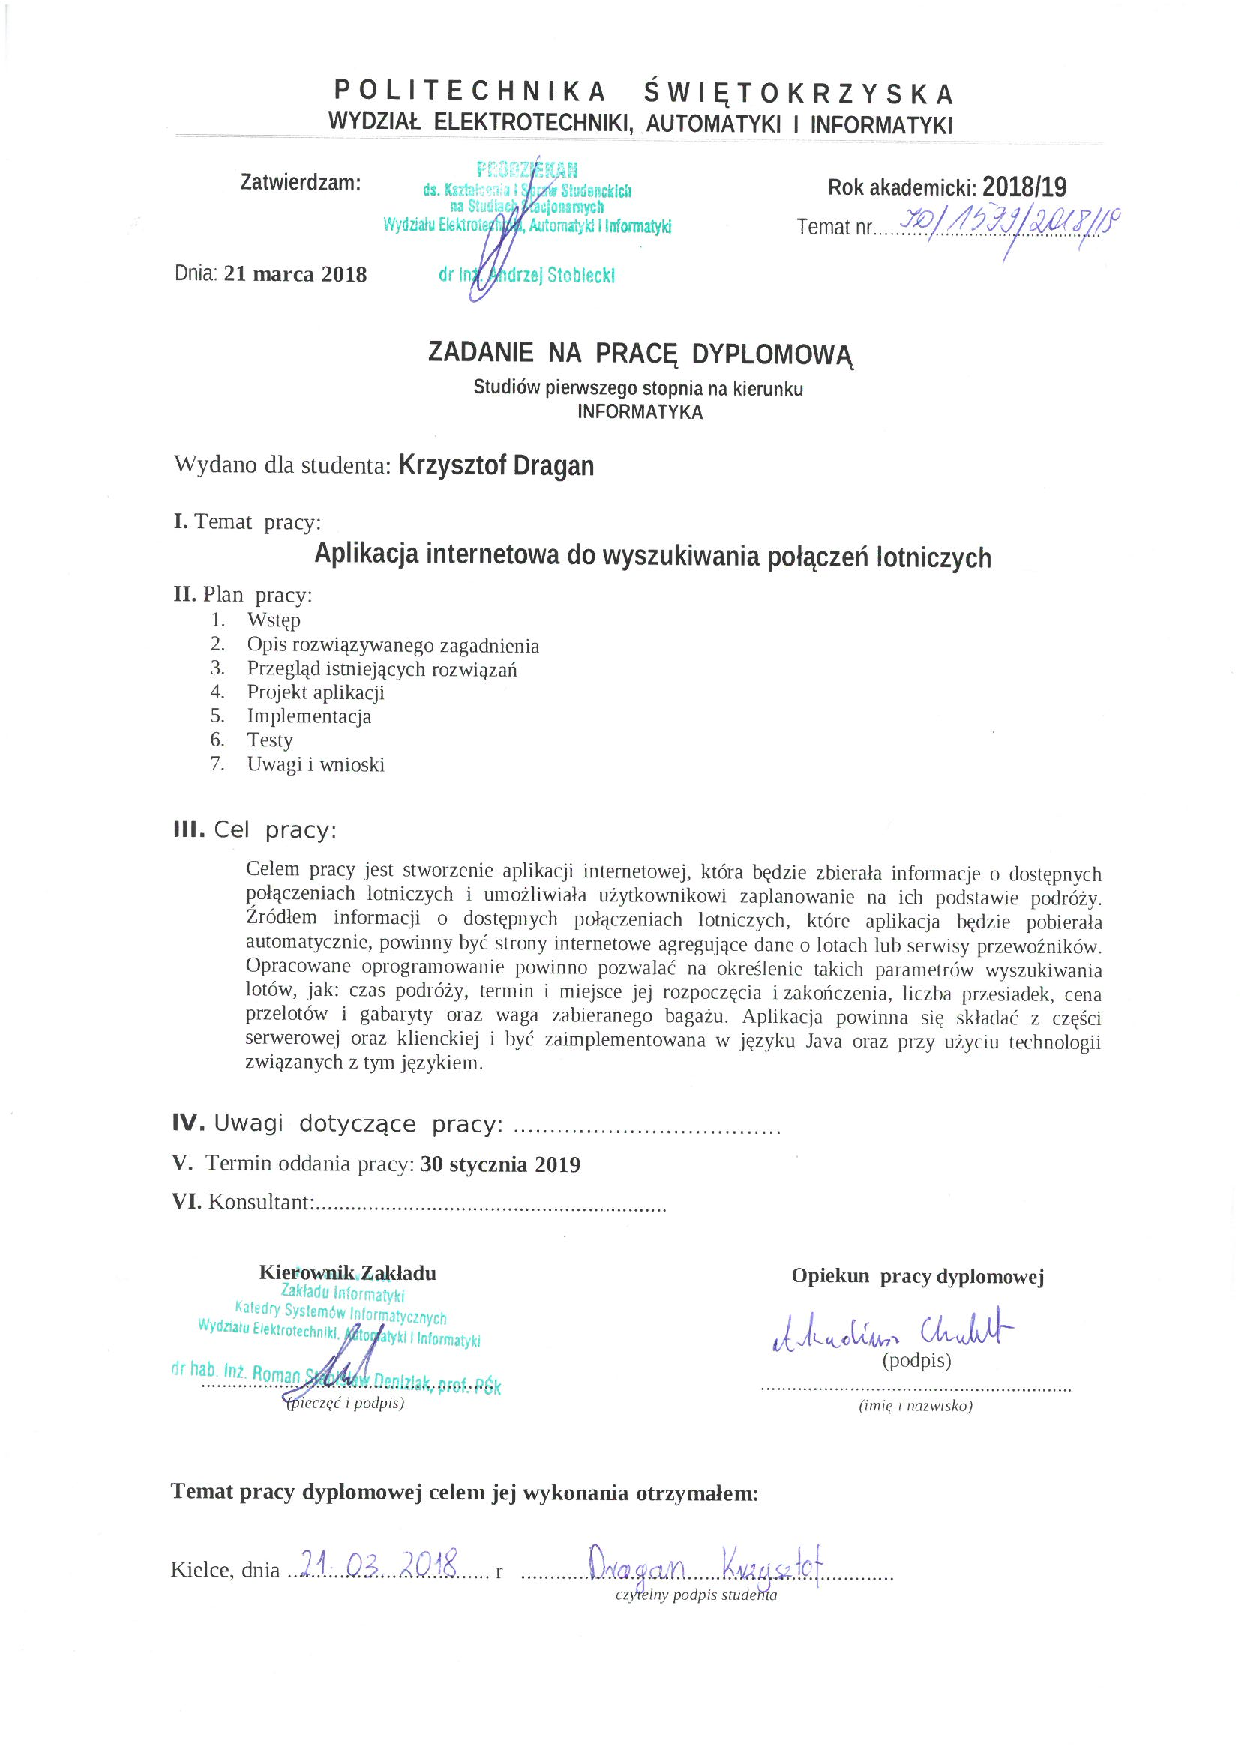
\includepdf[pages=-]{docs/zadanie.pdf}

% --------------------------------------------
% ---------------- Oświadczenie --------------
\afterpage{\blankpage}
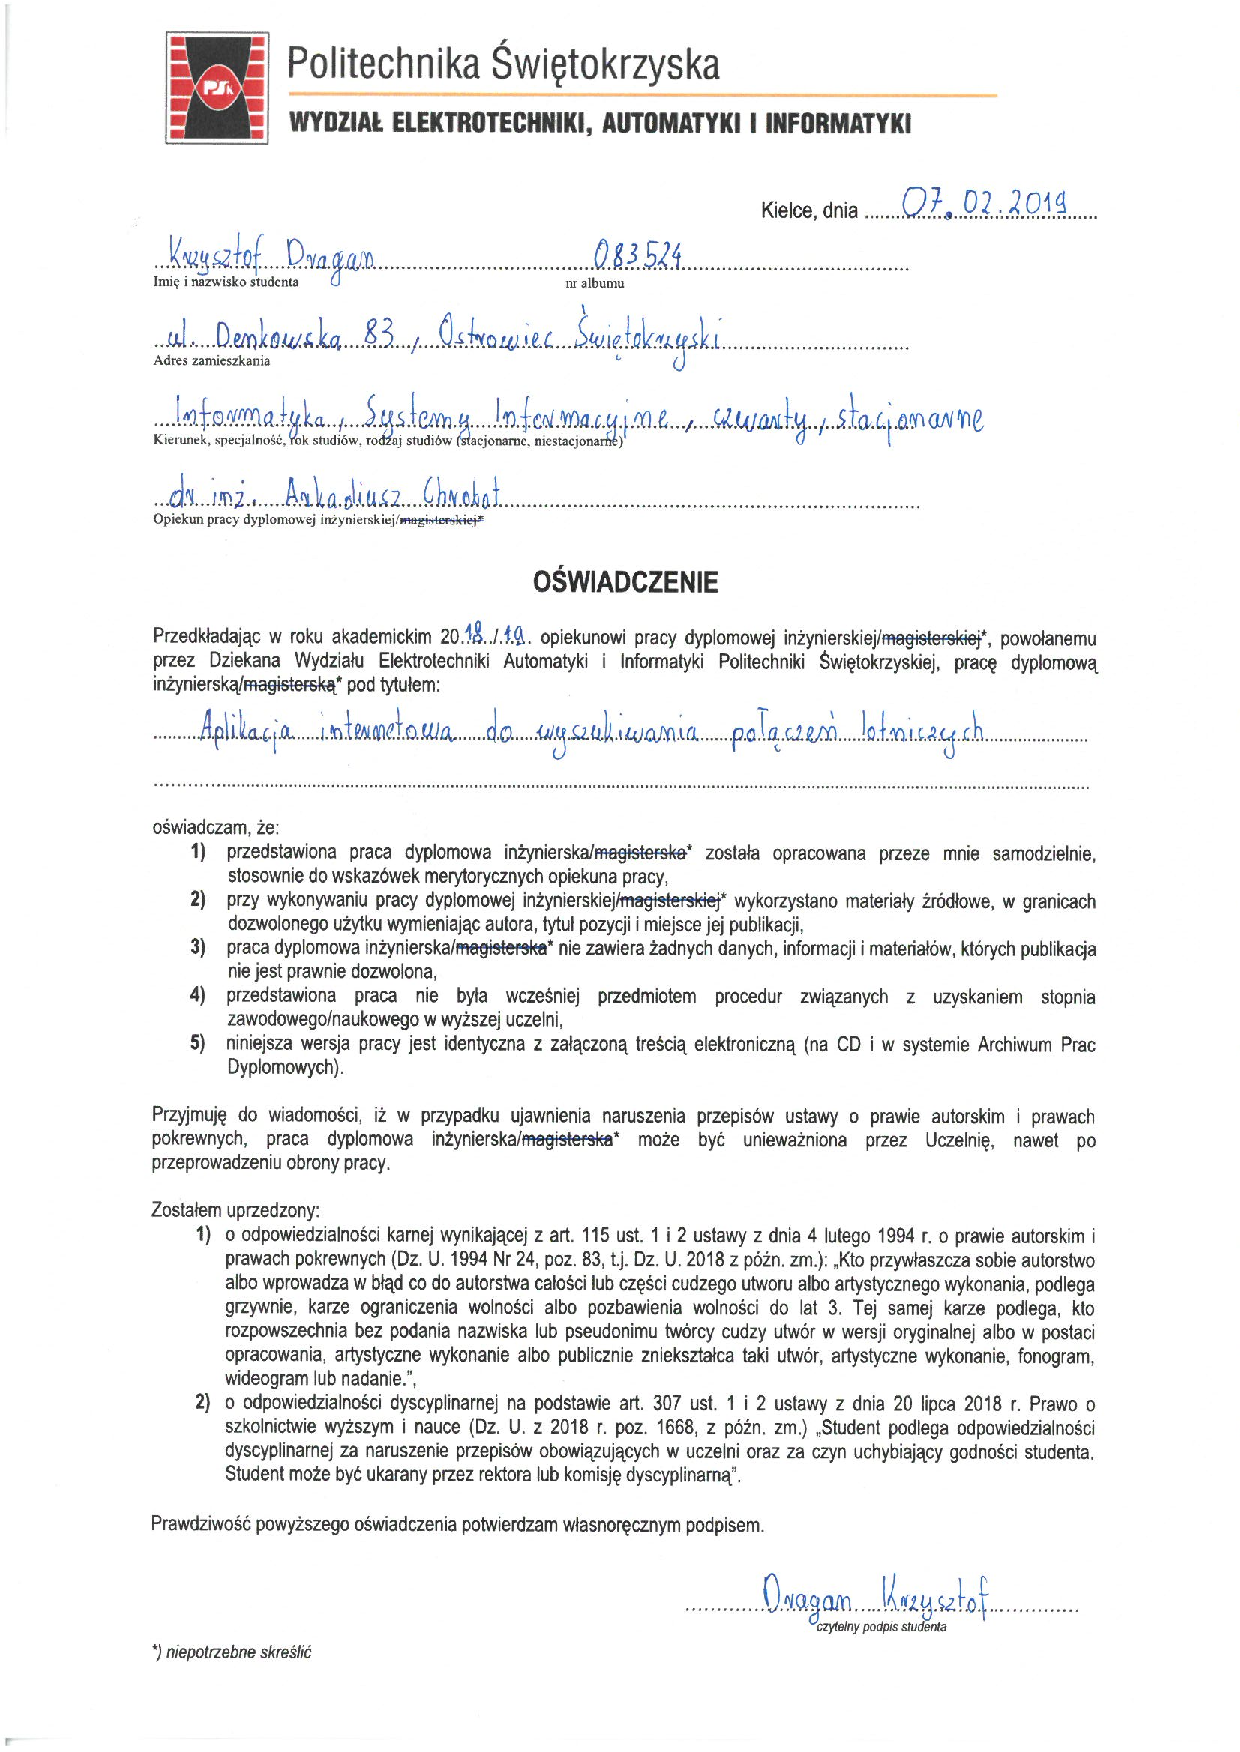
\includepdf[pages=-]{docs/oswiadczenie.pdf}  

% --------------------------------------------
% --------------- Streszczenie ---------------
\newpage
\thispagestyle{empty}
\begin{center}
	{\fontsize{14pt}{12pt}\selectfont
		\textbf{Aplikacja internetowa do wyszukiwania połączeń lotniczych}}
\end{center}

\begin{flushleft}
	{\fontsize{14pt}{12pt}\selectfont
		\textbf{Streszczenie}}\\
	\vspace{1cm}
\tab Celem niniejszej pracy było opracowanie aplikacji internetowej która pozwoliłaby na wyszukiwanie połączeń lotniczych korzystając z danych zawartych na stronach internetowych przewoźników bądź z innych centr danych. Aplikacja została podzielona na część kliencką oraz serwerową. Klient został napisany przy użyciu technologii Angular 6, natomiast część serwerowa w technologii Java 10. W pracy znajduje się opis architektury stworzonej aplikacji, modułu wyszukiwania połączeń lotniczych a także zagadnień teoretycznych związanych z projektowaniem interfejsu użytkownika dla przeglądarki internetowej.
\end{flushleft}
\vspace{0.5cm}
Słowa kluczowe: Java, Angular 6, REST, programowanie obiektowe, protokół HTTP, programowanie funkcyjne

\vspace{1.5cm}

\begin{center}
	{\fontsize{14pt}{12pt}\selectfont
		\textbf{A web application to search for flight connections}}
\end{center}

\begin{flushleft}
	{\fontsize{14pt}{12pt}\selectfont
		\textbf{Summary}}\\
	\vspace{1cm}
\tab The purpose of thesis was to build a web application, which will be able to search flight connections using data included on air websites or others data sources. Application was divided into two parts: client and server. Client was implemented using technology of Angular 6, whereas server in Java 10 technology. Description of architecture built application, module of air connections searching and theoretical issues related to building user interface for web application are included in this thesis. 
\end{flushleft}
\vspace{0.5cm}
Keywords: - Java, Angular 6, REST, Object Oriented Programming, HTTP Protocol, Functional Programming
\afterpage{\blankpage}

% ---------------- Spis Treści ---------------
\renewcommand{\contentsname}{Spis treści}
\newpage
\pagenumbering{arabic}
\setcounter{page}{9}
% Ustawia numerację strony od aktualnej na numer 9
\tableofcontents
% ------------------- Wstęp ------------------
\newpage
\chapter*{Wstęp}
\addcontentsline{toc}{chapter}{Wstęp}
Celem pracy było stworzenie aplikacji internetowej umożliwiającej wyszukiwanie połączeń lotniczych. Do zrealizowania tego celu potrzebne było dogłębne zbadanie problemów związanych z tym zagadnieniem. Pierwszym krokiem była analiza dostępnych źródeł danych o połączeniach lotniczych. Nie było to zadanie łatwe, tylko niektórzy przewoźnicy udostępniają swoje dane lotnicze na zewnątrz. Oprócz stron przewoźników istnieją też specjalne centra chmurowe gromadzące informacje o połączeniach lotniczych, jednakże w przeważającej części firmy reprezentujące te centra pobierały opłaty za możliwość korzystania z ich serwisów. Do zrealizowania celu wymienionego w pierwszym zadaniu posłużyła usługa chmurowa firmy FlightLookup która udostępniała zarejestrowanemu użytkownikowi jej dane w limicie 500 żądań protokołu HTTP na miesiąc. Oprócz tego do zrealizowania pracy zgodnie z założonymi wymaganiami potrzebne były źródła udostępniające informacje o liniach lotniczych, wymiarach i wagi bagażu podróżnego oraz cen przelotów. Kolejnym problem było poradzenie sobie z różnymi formatami danych które pozyskiwała część serwerowa. Deserializacja i serializacja danych odbywała się pomiędzy formatami: XML, JSON, HTML, CSV oraz obiektem języka Java. Dokładniejszy opis tego problemu znajduje się w rodziale Implementacja. Ważną kwestią była też wydajność aplikacji, czas odpowiedzi powinien być dla użytkownika jak najmniejszy. Kod źródłowy modułu zbierającego dane był odpowiednio przygotowany do wykonania tego zadania z jak najlepszym efektem. Zadbano o wyeliminowanie fragmentów kodu które mogłyby opóźnić odpowiedź aplikacji. Ponadto w pracy został zaimplementowanie mechanizm cachowania danych aby w przypadku gdy na przykład konkretny lot był wyszukiwany wiele razy, informacja o nim została zwrócona o wiele szybciej niż standardowo. \\
Aplikacja została podzielona na dwie części: część serwerową oraz kliencką.
Pierwsza część została stworzona w języku programowania Java w wersji 10.
Oprócz standardowego pakietu oprogramowania i narzędzi dostarczonego w JDK (Java Development Kit) zostały dodane biblioteki takie jak: Spring, Apache commons-io, Apache-csv czy też OkHttp. Biblioteka Spring jest odpowiedzialna w pracy za funkcjonowanie serwera udostępniającego dane oraz obsługę żądań sieciowych. Pozostałe biblioteki pomogły w procesie deserializacji i serializacji różnych formatów danych przychodzących do części serwerowej.
\newpage
Oprócz samego rozwiązania zbierającego dane o połączeniach lotniczych potrzebny był internetowy interfejs użytkownika który umożliwiał by prezentowanie danych w przyjemny dla użytkownika sposób. Do tego zadania, a więc zadania stworzenia częśći klienckiej wybrano technologię Angular 6. Angular jest platformą opartą na języku TypeScript która razem w połączeniu ze stronami HTML oraz arkuszami stylów CSS pozwoliła na stworzenie responsywnego interfejsu, co na obecnym rynku internetowym jest dużą zaletą. Zadaniem części klienckiej było odebranie danych od części serwerowej a następnie pokazanie ich w przeglądarce internetowej. Zewnętrznymi bibliotekami w tej części były Angular Material oraz Bootstrap. Przyspieszyły one budowanie komponentów interfejsu.
Kolejnym ważnym krokiem w pisaniu tej pracy było zaimplementowanie testów jednostkowych oraz integracyjnych które pozwoliłby na automatyczne sprawdzenie aplikacji pod względem wymaganych funkcjonalności zawartych w założeniach. Dopiero poprawne zakończenie wszystkich testów pozwoliło uznanie części praktycznej pracy za skończoną.

\newpage
\chapter{Opis rozwiązywanego zagadnienia}
Głównym zagadnieniem podjętym w pracy było znalezienie sposobu na pozyskanie realnych danych o połączeniach lotniczych które można by było zaprezentować w kompleksowym interfejsie oraz we względnie optymalnym czasie dla użytkownika powstałej aplikacji.
Zagadnienie to można podzielić na 3 części:
\begin{itemize}[noitemsep,topsep=0pt]
\item Znalezienie źródeł danych o połączeniach lotniczych
\item Parsowanie różnych rodzajów danych
\item Zapewnienie dobrej wydajności podczas wyszukiwania połączeń lotniczych
\end{itemize}
Części te zostaną opisane w podrozdziałach bieżącego rozdziału.

\section{Źródła danych o połączeniach lotniczych}
Największą trudnością podczas pisania pracy było znalezienie odpowiednich zasobów danych który nie byłyby płatne oraz które zapewniałyby rzetelne i sprawdzone dane lotnicze. Poszukiwania zaczęto od złożenia podań do centr danych o dostęp do ich zasobów. Większość z nich wymagała opłaty za swoje usługi które sięgały nawet 10000\$. Niektóre z nich oferowały jednak darmowy dostęp do ich zasobów jednak był to dostęp limitowany. Na potrzeby pracy wybrano serwis FlightLookup jako głównego dostawcę danych, informacje przez niego dostarczone stanowiły lwią część odpowiedzi serwera. Darmowy dostęp jest limitowany 500 zapytaniami w trakcie miesiąca.
\vspace{1.0cm}
\begin{figure}[!ht]
\centering

\includegraphics[scale=0.4, keepaspectratio]{flightlookup.png}
\caption{Portal serwisu FlightLookup}
\label{fig:flightlookup}
\end{figure}
\newpage
Dodatkowymi źródłami danych były:
\begin{itemize}[noitemsep,topsep=0pt]
\item Skyscanner - serwis udostępniające średnie ceny przelotów w określonym przedziale czasowym oraz informacje dotyczące dozwolonego bagażu
\item Aviation Edge - usługa chmurowa udostępniające dane o liniach lotniczych 
\item ourairport.com - strona internetowa umożliwiające pobranie danych o większości lotnisk na świecie
\end{itemize}

\section{Parsowanie różnych rodzajów danych}
Dane dostarczone przez zewnętrzne serwisy prezentowały swoją treść w różnych formatach. Aby zebrać pełną odpowiedź serwera należało w pierwszym kroku sparsować pojedyncze elementy a następnie zbudować z nich obiekt języka Java. Parsowanie zaczynało się od odebrania danych z serwisu FlightLookup w postaci XML (eXtensible Markup Language). Do zrealizowania tej czynności posłużono się zewnętrzną biblioteką jackson-dataformat-xml która efektywnie przełożyła obiekty XML na odpowiedni obiekty Javy.
%tutaj załączyć kod xml z odpowiedzą serwera FlightLookup

\begin{lstlisting}[language=XML, caption=Przykładowe dane w XML]
    <FlightDetails TotalFlightTime="PT3H35M"
                   TotalMiles="931"
                   TotalTripTime="PT4H25M"
                   FLSDepartureDateTime="2018-11-15T06:40:00"
                   FLSDepartureTimeOffset="+0100"
                   FLSDepartureCode="WAW"
                   FLSDepartureName="Warsaw"
                   FLSArrivalDateTime="2018-11-15T10:05:00"
                   FLSArrivalTimeOffset="+0000"
                   FLSArrivalCode="LHR"
                   FLSArrivalName="London Heathrow"
                   FLSFlightType="Connect"
                   FLSFlightLegs="2"
                   FLSFlightDays="...4..."
                   FLSDayIndicator=""
                   >
\end{lstlisting}

\newpage
Informacje o liniach lotniczych dostarczane były w postaci JSON (JavaScript Object Notation). Do sparsowania ich posłużono się biblioteką Gson organizacji Google. Dzięki niej konwersja obiektu JSON do obiektu Java odbywała się w jednej linii kodu. W ten sam sposób odbywało się parsowanie danych zawierających ceny przelotów.\\
Ostatnim formatem danych który wymagał sparsowania był HTML (Hypertext Markup Language). Informacje przez niego opisane dotyczyły wymiarów oraz wagi bagażów dozwolonych na określonej linii lotniczej. Do wykonania tego zadania posłużyła zewnętrzna biblioteka Jsoup. Dedykowana dla języka Java, z gotowym pakietem oprogramowania bardzo dobrze poradziła sobie z parsowaniem treści HTML.

\section{Wydajność wyszukiwania}
Wyszukiwanie tak złożonych jak informacje o połączeniach lotniczych a następnie parsowanie ich niesie za sobą pewne konsekwencje. Są to konsekwencje czasownik, użytkownik powinien otrzymać interesującą go treść w czasie jak najkrótszym. W celu optymalizacji wydajności aplikacji wprowadzono mechanizmy skracające czas odpowiedzi części serwerowej. Dla zbierania danych dotyczących lotnisk oraz bagażów wprowadzono rozwiązania polegające na pobieraniu pełnych zasobów tych danów do bazy danych lub do pliku znajdującego się na serwerze. Pozwoliło to na pominięcie opóźnienia sieciowego związanego z potencjalną koniecznością pobierania tych danych ze stron lub zewnętrznych baz danych. \\
Kolejnym rozwiązaniem było wprowadzenia stylu programowania funkcyjnego w kluczowych elementach części serwerowej które odpowiadały za wyszukiwanie połączeń lotniczych. Programowanie funkcyjne wprowadzone w Javie 8 pozwala skrócić operacje po stronie wirtualnej maszyny Javy a więc też zaoszczędzić cenne milisekundy w trakcie wyszukiwania lotów.
Ostatnim mechanizmem był moduł cachowania danych. Jego przeznaczeniem jest skracanie czasu odpowiedzi dla określonych zapytań do części serwerowej które są zwielokrotnione i wywoływane przez wielu użytkowników. Wykonując operacje wyszukiwania lotów, moduł wyszukiwania sprawdza czy w cache'u znajdują się poszukiwanie operacje. Jeśli tak zwraca je użytkownikowi, jeśli nie wyszukuje loty standardowym sposobem a wynik zapisuje do cache'u. Cache przetrzymuje w sobie do 100 zapytań.
\newpage
\chapter{Przegląd istniejących rozwiązań}
Analiza istniejących rozwiązań aplikacji wyszukujących połączeń lotniczych pozwoliła nadać pracy bardziej precyzyjne wymagania oraz zaprojektować jej ogólny przebieg. W internecie można znaleźć wiele aplikacji o podobnych lub takich samych funkcjonalnościach jak tworzona praca. W tym rodziale zostaną opisane najbardziej znane wyszukiwarki lotów dostępnych na rynku. 
\section{Wyszukiwarka lotów Skyscanner}
Pierwszym przykładem została aplikacja internetowa Skyscanner. Jest to wyszukiwarka lotów, która umożliwia użytkownikom szukanie lotów według ceny i lokalizacji. Oprócz funkcji wyszukiwania lotów, Skyscanner oferuje opcje wyszukiwania hotelów blisko lotnisk oraz wypożyczenia auta w pobliżu lotniska docelowego. Aplikacja ta została stworzona oraz wdrożona w 2002 roku. Od tego czasu firma Ctrip która jest właścicielem tego produktu zatrudnia ponad 200 pracowników. Warto wspomnieć o jej innej usłudze która udostępnia dane o połączeniach lotniczym zewnętrznym firmom i deweloperom. Jej dane były brane pod uwagę w czasie szukania źródeł danych lecz Skyscanner wymaga dużych opłat za swoje usługi, w warunkach akademickich niemożliwe było z ich skorzystanie.
 Aplikacja ta jest dostępna w ponad 30 językach oraz używana przez 60 milionów użytkowników miesięcznie. Aplikacja wiele razy nagradzana była za swoją funkcjonalność i użyteczność użytkownikom. Skyscanner znajduje się pod adresem: \url{https://www.skyscanner.net/}

\vspace{1.0cm}
\begin{figure}[!ht]
\centering

\includegraphics[scale=0.4, keepaspectratio]{skyscanner.png}
\caption{Logo aplikacji Skyscanner}
\label{fig:skyscanner}
\end{figure}

 
\newpage
Na swojej stronie internetowej na pierwszy rzut oka można zauważyć panel wyszukiwania lotów.


\newpage
\section{Wyszukiwarka lotów Google Flights}



\end{document}